\documentclass[dvipdfmx]{jarticle}
\usepackage{tikz}
\usetikzlibrary{automata,calc}
\usepackage{url}
\pagestyle{empty}
\begin{document}
\begin{flushright}
    \verb|2026/10/02|
\end{flushright}
\begin{center}
    {\bf\Large コンパイラ第1回演習課題}
\end{center}

\vspace*{5mm}

\begin{itemize}
    \item TACTの課題の添付としてPDFファイルを提出すること．
    \item レポートをPDFとして提出する方法は講義webサイト\footnote{\url{https://sites.google.com/sqlab.jp/26compiler/how-to-make-report}}を参照
    \item 提出期限：10月9日 23:55(JST)
\end{itemize}

\vspace*{5mm}

\begin{enumerate}
    \item 以下の無向グラフについて
          \begin{center}
              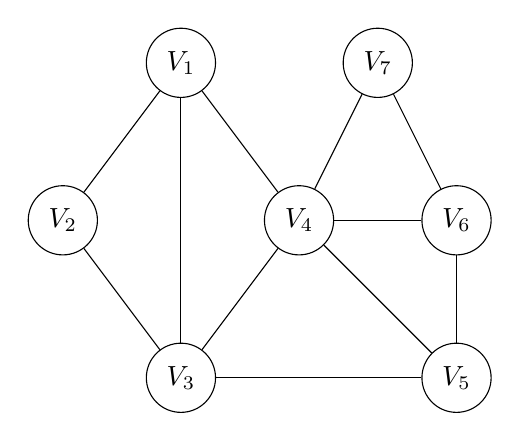
\begin{tikzpicture}
                  \node[state] (V1) at (1.5,4) {$V_1$};
                  \node[state] (V2) at (0,2) {$V_2$};
                  \node[state] (V3) at (1.5,0) {$V_3$};
                  \node[state] (V4) at (3,2) {$V_4$};
                  \node[state] (V5) at (5,0) {$V_5$};
                  \node[state] (V6) at (5,2) {$V_6$};
                  \node[state] (V7) at (4,4) {$V_7$};
                  \path[-] (V1) edge (V2) (V1) edge (V3) (V1) edge (V4)
                  (V2) edge (V3) (V3) edge (V4) (V3) edge (V5)
                  (V4) edge (V5) (V4) edge (V6) (V4) edge (V7)
                  (V5) edge (V6) (V6) edge (V7);
              \end{tikzpicture}
          \end{center}
          \begin{enumerate}
              \item 最大独立集合となりうる頂点の集合をすべてあげよ．
              \item このグラフは弦グラフの条件を満たすか？条件を満たす場合は，頂点の完全消去順序を示せ．満たさない場合は，その理由を示せ．
          \end{enumerate}
    \item 正の3の倍数を表す10進数の文字列の集合について $\{3,6,9,12,\cdots\}$
          入力アルファベットを$\{0,1,2,\cdots,9\}$としてこの集合を受理する受理するDFAを示せ．(ヒント：5状態のDFAで表現できる．)
          % \item $L\subseteq \{0,1\}^\ast$を以下の遷移図で表される有限オートマトン$M$で受理される言語とする．

          %       \begin{center}
          %           \begin{tikzpicture}[node distance=2cm,auto]
          %               \node[state,initial] (Q0) at (0,0) {$q_0$};
          %               \node[state] (Q1) at (2,1) {$q_1$};
          %               \node[state,accepting] (Q2) at (2,-1) {$q_2$};
          %               \path[->] (Q0) edge [loop above] node {0} ()
          %               (Q0) edge [above] node {1} (Q1)
          %               (Q1) edge [right] node {0} (Q2)
          %               (Q1) edge [above] node {1} (Q0)
          %               (Q2) edge [above] node {0} (Q0)
          %               (Q2) edge [loop right] node {1} ();
          %           \end{tikzpicture}
          %       \end{center}
          %       \begin{enumerate}
          %           \item $L^R=\{w^R\ \vert\ w\in L\}$とする．ここで，$w^R$は$w$を反転した語を表す．$L^R$ を受理するNFA $M^R$を構成せよ．
          %           \item $L''=\{w\ \vert\ w w^R\in L\}$とする．$L''$を受理するNFAを$M$と$M^R$を用いて構成せよ．
          %       \end{enumerate}
          %    \item 教科書27ページ　演習問題７
\end{enumerate}
\end{document}